%
\documentclass[a4paper,12pt,final]{article}
%
% import des differents packages
\usepackage[english,francais]{babel}
\usepackage[utf8]{inputenc}
\usepackage[T1]{fontenc}
\usepackage[pdftex]{graphicx}
\usepackage{setspace}
\usepackage{hyperref}
\usepackage[french]{varioref}
%
% pour régler les marges :
\usepackage[top=2.5cm,bottom=2.3cm,right=2cm,left=2cm]{geometry}
%
%
%
\newcommand{\reporttitle}{Extension évolutive d'un réseau hospitalier}     % Titre
\newcommand{\reportauthor}{\textsc{Massip} Thomas, \textsc{Roques} Nicolas, \textsc{Tosi} Émeric} % Auteur
\newcommand{\reportsubject}{Architecture de réseaux - B.E. Sujet A} % Sujet
\newcommand{\reportdate}{04 Novembre 2015} % Date
%
%
\newcommand{\HRule}{\rule{\linewidth}{0.5mm}}
\setlength{\parskip}{4ex} % Espace entre les paragraphes
%
%
\hypersetup{
    pdftitle={\reporttitle},%
    pdfauthor={\reportauthor},%
    pdfsubject={\reportsubject},%
    pdfkeywords={rapport} {B.E.} {Architecture de réseaux} {Sujet A}
}
%
%
\begin{document}
    %
    % Inspiré de http://en.wikibooks.org/wiki/LaTeX/Title_Creation
%
\begin{titlepage}
    %
    \begin{center}
        %
        \begin{minipage}[t]{0.48\textwidth}
            \begin{flushleft}
                
\includegraphics [width=50mm]{images/logo-univ.png}
                \\[0.7cm]
                \begin{spacing}{1.3}
                    \textsc{\LARGE Université Toulouse III Paul Sabatier}
                \end{spacing}
            \end{flushleft}
        \end{minipage}
        %
        %
        \begin{minipage}[t]{0.48\textwidth}
            \begin{flushright}
                
\includegraphics [width=50mm]{images/logo-stri.png}
                \\[0.7cm]
                \textsc{\LARGE Filière STRI}
            \end{flushright}
        \end{minipage}
        %
        \\[3.7cm]
        %
        %
        \textsc{\Large \reportsubject}\\[0.7cm]
        \HRule \\[0.7cm]
        %
        %
        {\huge \bfseries \reporttitle}\\[0.7cm]
        \HRule \\[8.5cm]
        %
        %
        \begin{flushleft} \large
            \emph{Auteurs :}\\
            \reportauthor
        \end{flushleft}
        %
        %
        \vfill
        %
        %
        {\large \reportdate}
    %
    \end{center}
%
\end{titlepage}

    \cleardoublepage % Dans le cas du recto verso, ajoute une page blanche si besoin
    %
    \tableofcontents % Table des matières
    \sloppy          % Justification moins stricte : des mots ne dépasseront pas des paragraphes
    \cleardoublepage
    %
    \section*{Introduction} % Pas de numérotation
\addcontentsline{toc}{section}{Introduction} % Ajout dans la table des matières

%
%

Une expansion d'une clinique, dédiée aux maladies des voies respiratoires, voit le jour à 50 mètres d'un des bâtiments déjà existant.
Nous sommes chargés de réaliser l'étude d'architecture réseau à implanter dans ce nouveau bâtiment.

%
%

Ce réseau devra répondre à une certaine tolérance aux pannes puisque utilisé à des fins médicales et nécessitera une interconnexion avec le bâtiment adjacent.
Dans l'architecture réseau actuelle le cœur de réseau et l'accès à Internet se trouvent dans le bâtiment adjacent.
Le déploiement de la nouvelle portion de réseau ne devra avoir aucune incidence sur le réseau déjà existant de la clinique.

%
%

Sur le nouveau bâtiment il est nécessaire de définir et prendre en compte les contraintes imposées par les personnes, les matériels et leurs usages.
Chaque étage est dédié à des usages différents :
\begin{itemize}
\item Le niveau -2 contient le parking et les vestiaires du personnel;
\item Le niveau -1 contient le service de radiologie, avec des salles de scanners et des blocs opératoires;
\item Le rez-de-chaussée contient la salle d'accueil et le local technique principal;
\item Le niveau 1 contient les bureaux du personnel et les salles de réunion;
\item Les niveaux 2 à 4 contiennent les chambres des patients.
\end{itemize}
On s'aperçoit que ces différences entre étages seront un point de départ important pour l'architecture du réseau :
certains équipements médicaux nécessitent d'être inter-connectés, d'autres ne doivent en aucun cas être parasités pour assurer leur fonctionnement.

%
%

    \cleardoublepage
    %
    \section{La première section}

%
\subsection{Une sous section}

On peut mettre des mots en \emph{italique},
en \textsc{petites Majuscules} ou
en \texttt{largeur fixe (machine à écrire)}.

Voici un deuxième paragraphe avec une formule mathématique simple : $e = mc^2$.

Un troisième avec des \og guillemet français \fg{}.


%
\subsubsection{Écrire en anglais}

\foreignlanguage{english}{Do you speak French? Does anybody here speak french?}


%
\subsection{Listes}

\begin{itemize}
\item Liste classique ;
\item un élément ;
\item et un autre élément.
\end{itemize}
\vspace{\parskip} % espace entre paragraphes

\begin{enumerate}
\item Une liste numéroté
\item deux
\item trois
\end{enumerate}
\vspace{\parskip}

\begin{description}
\item[Description] C'est bien pour des définitions.
\item[Deux] Ou pour faire un liste spéciale.
\end{description}
\vspace{\parskip}


%
\subsection{Références}

Voici une référence à l'image de la figure \ref{latex} page \pageref{latex} et une autre vers la partie \ref{p2} page \pageref{p2}.

On peut citer un livre\,\up{\cite{lpp}} et on précise les détails à la fin du rapport dans la partie références.


%
\subsection{Note de bas de page}

Voici une note\,\footnote{Texte de bas de page} de bas de page.
Une deuxième\,\footnotemark{} déclarée différemment.
La même note\,\footnotemark[\value{footnote}] que précédemment.

\footnotetext{Il a deux références vers cette note}


%
\subsection{Figure}

\begin{figure}[!ht]
    \center
    
\includegraphics[]{./images/LaTeX_logo.png}
    \caption{latex | taille original}
    \label{latex}
\end{figure}

\begin{figure}[!ht]
    \center
    
\includegraphics[width=0.5\textwidth]{./images/LaTeX_logo.png}
    \caption{latex | 50\% de la largeur de la page}
\end{figure}




%~ ---------------------------------------------------------------------
%~ ---------------------------------------------------------------------
%~ ---------------------------------------------------------------------


%~ Contexte

%~ La question essentielle se pose : Comment structurer la nouvelle architecture réseau du nouveau bâtiment hospitalier ?
%~ En effet, l’objectif principal d’évolution est de structurer l’architecture comme indiqué ci-dessous :

%~ Cœur
%~ Distribution
%~ Accès

%~ Ces trois structures sont indispensables afin de bien consolider l’architecture hospitalier. L’objectif principal est d’assurer un service performant et sécurisé pour le personnel et les patients. Le réseau dans un hôpital ne demande pas spécialement de performances de débit, mais demande plus particulièrement des solutions fonctionnelles,  et sécurisées.

%~ Pour la couche accès, ici l’objectif est de raccorder différents équipements hétérogènes tels que les téléphones le Wifi, les tablettes etc…Dans cette couche nous trouverons différents VLAN pour chaque entités d’utilisateurs (personnels et visiteurs)

%~ Pour la couche distribution, permet l’agrégation de flux homogènes tels que Ethernet et la capacité en commutation de circuits.

%~ Pour la couche cœur de réseau, il sera préférable de bien différentier nos différents réseaux du personnel et des visiteurs (patients)
%~ Dans cette partie des protocoles seront mis en place pour assurer les structurations architecturales de l’ensemble du réseau.

%~ Ces objectifs permettront d’assurer une fiabilité du réseau du par ses différents échanges

%~ Plusieurs hypothèses peuvent répondre au cahier des charges demandé. Cependant, notre éventuelle solution se porte principalement sur les critères suivants :
%~ -Budget
%~ -Topologie réseau
%~ - Le temps de l’évolution.

%~ Nous avons décidé de se focaliser principalement sur le nouveau bâtiment. En fonction de la description de l’existant.
%~ La première idée que l’on se pose est de savoir par quel lien nous allons relier les deux bâtiments ? Le choix de la fibre monomode semble le plus opportun. Une redondance de lien est nécessaire pour
%~ La seconde idée se pose à la redondance du cœur du réseau. Un cœur de réseau déjà existant à l’ancien bâtiment doit être dupliqué au nouveau bâtiment, avec un certain niveau de sécurité offrant la TOIP, l’accès à internet, la sauvegarde et l’accès à la base de données.
%~ La troisième idée permet d’offrir un accès sans fil Wifi au personnel afin de consulter les ressources en toute mobilité. Les patients également auront accès à un réseau sans fil différent.
%~ La quatrième idée est d’assurer la qualité de service (QOS), chaque étage dispose d’un local dédié permettant de fournir l’accès aux ressources réseaux. Les étages seront assurés par des protocoles de gestion.

%~ Hypothèse future :
%~ L’ensemble de l’architecture de l’ancien bâtiment se coordonne aux éventuelles solutions que nous mettrons en place au nouveau bâtiment. Cependant si le projet souhaite évoluer d’ici quelques années et que le budget est conséquent, une remise à niveau de l’architecture de l’ancien bâtiment semblerait importante.
%~ Un redimensionnement du réseau
%~ Remise d’actualité des câbles
%~ Virtualisation du PABX, ou mise en place de la TOIP
%~ Virtualisation totale des serveurs et cœur de réseau.
%~ Sauvegarde externalisée.
%~ Un réseau Wifi séparé pour le personnel et les visiteurs
%~ Matériels fournit (tablettes, postes, et téléphones IP)


    \cleardoublepage
    %
    \section{Architecture Logique}

Pour répondre au besoin présenter ci-dessus, nous allons d'abord établir une architecture logique de l'infrastructure.
Cela permet de représenter les équipements ainsi que leur interconnexion.
Elle a pour but d'identifier les différents rôles et services de chaque équipement à installer.
C'est cette architecture qui justifie la qualité du réseau que nous proposons vis à vis des services attendus.

%
%
\subsection{Couches logiques}

\begin{figure}[!ht]
    \center
    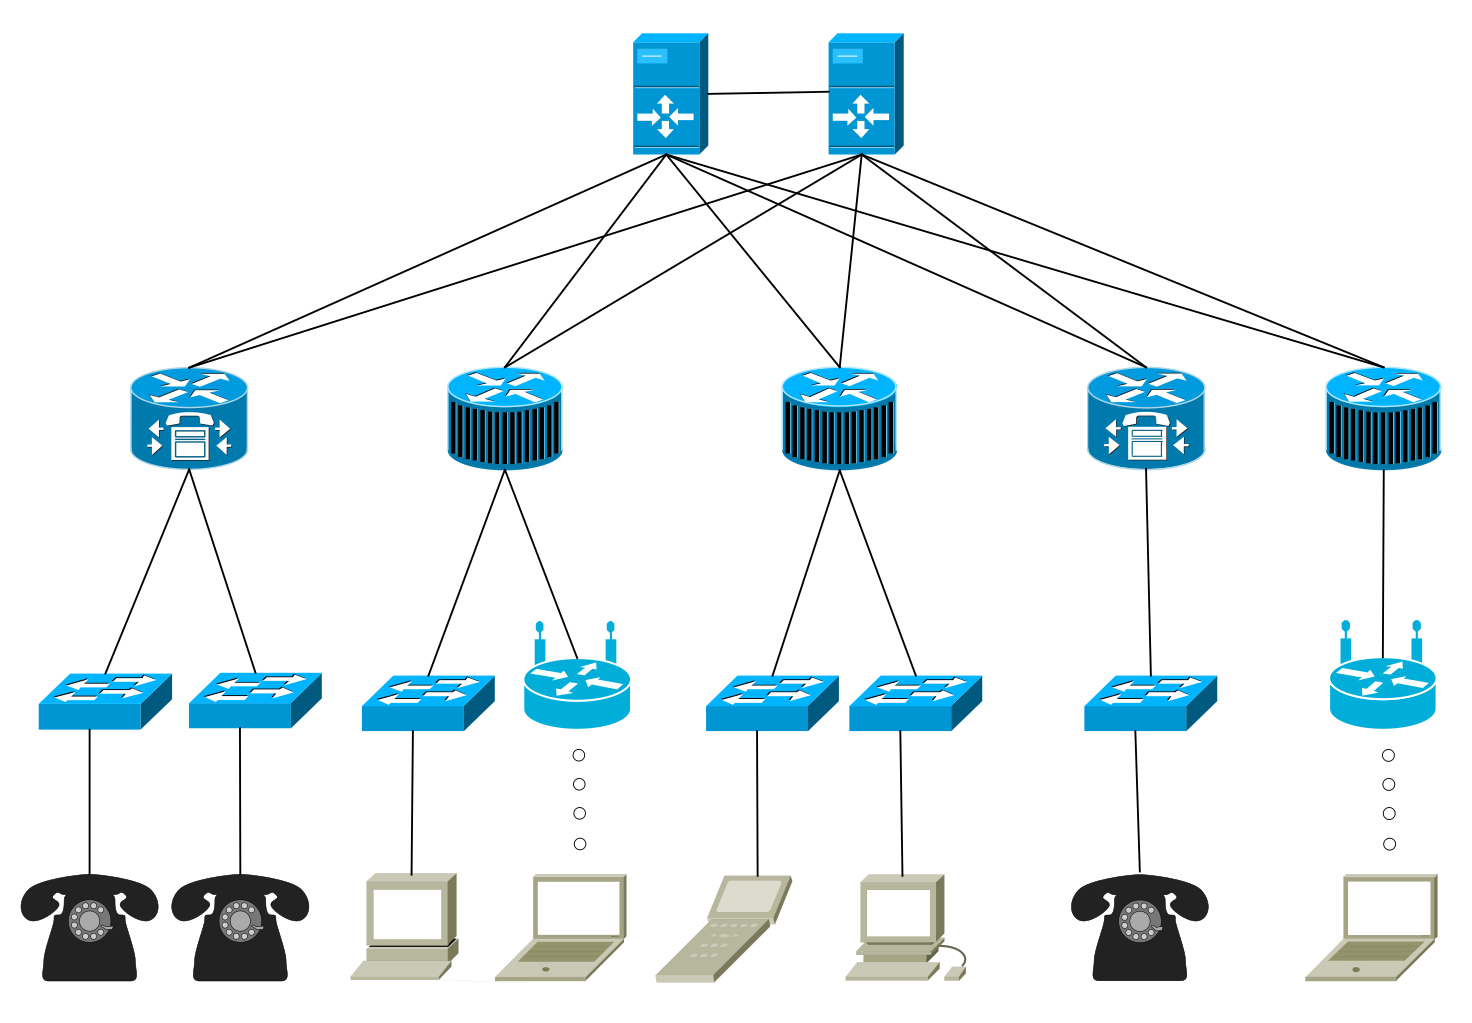
\includegraphics[width=1\textwidth]{./images/schema-logique.png}
    \caption{Schéma logique hiérarchique du réseau}
\end{figure}

%
    \cleardoublepage
%

\subsubsection{Couche coeur}
C’est la couche supérieure.
Son rôle est de relier entre eux les différents segments du réseau, par exemple les sites distants, les LANs ou les étages d'une société.
Dans notre cas le coeur du réseau sera constitué de deux routeurs.

\subsubsection{Couche distribution}
Cette couche consiste à router, filtrer autoriser ou non les paquets.
C'est a ce niveau que nous allons donc crée des VLANs sur les routeurs afin de délimiter l'étendu du réseau.
Nous décidons de faire deux VLAN principaux : VLAN Interne, VLAN Visiteur.

\subsubsection{Couche accès}
Cette couche est la dernière avant de transmettre le paquet à l'hôte.
Elle ne contient que des commutateurs qui permettrons de relayer l'information.

\subsubsection{Couche hôtes}
Il s'y trouve ici les différents types de terminaux .Tels que les terminaux portatifs, les ordinateurs fixe, les appareils médicaux( Scanner, radio etc).

%
    \cleardoublepage
%
%
\subsection{VLANs}

Nous avons décider de séparer le réseau interne avec celui des visiteurs pour une raison de qualité de service.
Le besoin et la sécurité ne sont pas la même entre ses deux réseaux.

%
%
\subsubsection{VLAN interne}

Le VLAN Interne est divisé à l'intérieur en 3 VLANs.

VLAN Données-Interne:
Il regroupe les différents équipements des bureaux administratif, des salles de réunions et de l'accueil.

VLAN VoIP-Interne:
Il regroupe tous les équipements téléphoniques du personnel de l'hôpital, afin d'assurer une qualité de service vis a vis de la communication dans l'hôpital.

VLAN Médical:
Il regroupe tous les équipements médicaux tels que les scanners , IRM et autre machines a usage médicales.
Il y a aussi les informations des patients stocké dans celui-ci.

%
%
\subsubsection{VLAN visiteur}

Le VLAN Visiteur est lui divisé en 2 VLANs.

VLAN Données-Visiteur:
Il regroupe toutes les données qui seront émises par le visiteur a l'aide de son téléphone portable ou tablette par exemple.

VLAN VoIP-Visiteur:
Il regroupe  tous les équipements téléphoniques fixe installer dans les chambres pour les patients.



%
%
\subsection{A FINIR}

adressage + plan nommage
faire des sous réseau

Etages
VLAN
plage d’adresse
n0-n4
VLAN DonnéesInterne
10.2.0.0/16
Tous
VLAN Médical
10.1.0.0/16
Tous
VLAN VoIPInterne
10.0.0.0/16
n2-4
VLAN
VoIPVisiteur
10.128.0.0/16
n0-4
VLAN DonnéesVisiteur
10.129.0.0/16


%
%

    \cleardoublepage{}
    %
    \section{Architecture matérielle du réseau}

%
%
\subsection{Architecture physique}

Après avoir vu l'architecture logique de notre réseau, nous pouvons maintenant établir l'architecture physique du réseau ainsi que le nombre d'équipements requis.

Tout d'abord, les deux bâtiments sont reliés à l'aide de deux fibres optiques de 100m (afin d'effectuer de la redondance en cas de coupure d'une de ces deux fibres) que l'on intègre dans le faux plafond du tunnel reliant les deux bâtiments.
Les fibres sont relié aux routeurs qui ce situant au N0. Elles sont connectées au routeur à l'aide de connecteur SFP+.

Le niveau -1 est le niveau où les scanners, radio s'effectuent ainsi que les opérations. Comme vue précédemment, il n'y a ni de WiFi, n'y d'accès à internet à ce niveau.
Les équipements médicaux étant branchés directement sur les ordinateurs a l'aide de câble console, on relie les ordinateurs ainsi que les téléphones au commutateur du niveau -1 situé dans un local prévu à cet effet.
De ce fait, les terminaux du niveau -1 font partie du VLAN Médical.

Au niveau 0, une salle est entièrement dédié aux équipements réseau. Cette salle contient une armoire. On y installe deux routeurs, deux lames serveur qui sont sur deux machines différentes, un NAS, un onduleur afin de palier aux pannes de courant ainsi que trois commutateurs.
Deux commutateurs de coeur de 24 ports où sont relié tous les équipements de l'infrastructure réseau et un commutateur 24 ports concernant le raccordement des terminaux du niveau 0.
Tous les équipements dans la salle sont doublés afin de garantir une haute disponibilité.

Il y a aussi  trois bornes WiFi, une fournissant internet pour les visiteurs et deux autres pour le personnel.
La borne WiFi fournissant internet pour les visiteurs fait partit du VLAN DonnéesVisiteur.
Les téléphones pour l'accueil et les bureaux administratif font partie du VLAN VoIPInterne.
Les ordinateurs et les bornes WiFi destinés aux personnels eux font partie du VLAN Données-Interne.

Le niveau 1 contient uniquement des terminaux faisant partit du VLAN Interne. Les terminaux téléphoniques font partie du VLAN VoIP-Interne, les ordinateurs et les deux bornes WiFi du VLAN Données-Interne. Tous les terminaux sont raccordés sur deux commutateurs de 24ports qui se situent dans le local de l'étage prévue à cet effet. Les équipements téléphoniques sont raccordés à un commutateur et les autres types de terminaux tels que les ordinateurs, bornes WiFi et prises RJ45 supplémentaires sur le deuxième commutateur.


Pour les niveaux de 2 à 4, on place une borne WiFi afin de fournir Internet aux patients. Cette borne fait partit du VLAN Données-Visiteur. Les téléphones pour les patients se situant dans chaque chambres font partie du VLAN VoIP-Visiteur.
Pour les médecins, infirmières, deux bornes WiFi sont mise en place et deux ordinateurs. Ces terminaux font partie du VLAN Données-Interne.
Deux téléphones sont aussi présent pour le personnel, ils font partie du VLAN VoIP-Interne.
Tous les terminaux sont raccordés à un commutateur. Du au grand nombre de terminaux à ces étages, deux commutateurs seront mis en place. Pour une question d'installation et de maintenance, tous les téléphones sont relié à un commutateur et les autres terminaux de type ordinateur et borne sont reliés au deuxième commutateur.

Les commutateurs se trouvant aux étages sont reliés directement sur les  deux commutateur de coeur qui se situe dans la salle du niveau 0.

Les téléphones et les bornes WiFi sont alimentés en PoE pour éviter d'installer des prises électriques à coté de ceux-ci.
Tous les raccordements sont fait à l'aide de câbles Ethernet SSTP catégorie 6 RJ45 sans halogène.


%
%
\subsection{Détails par étage}

    \begin{center}
        \begin{tabular}{|l|p{10cm}|r|}
          \hline
            Étages  &   Équipements    &   Prises RJ45 \\
          \hline
            N -1    &
            \begin{itemize}
                \item 6 Téléphones
                \item 8 Ordinateurs
                \item 1 commutateur 24ports
            \end{itemize}
            &   14 + 6 libres \\
          \hline
            N 0    &
            \begin{itemize}
                \item 3 Bornes WiFi
                \item 8 Téléphones
                \item 8 Ordinateurs
                \item 2 routeurs
                \item 2 Pare-feux logique
                \item 3 commutateur 24ports
                \item 1 NAS
            \end{itemize}
            &   16 + 4 libres \\
          \hline
            N 1    &
            \begin{itemize}
                \item 2 Bornes WiFi
                \item 9 Téléphones
                \item 9 Ordinateurs
                \item 2 commutateur 24ports
            \end{itemize}
            &   18 + 9 libres \\
          \hline
            N 2 à 4    &
            \begin{itemize}
                \item 3 Bornes WiFi
                \item 17 Téléphones
                \item 2 Ordinateurs
                \item 2 commutateur 24ports
            \end{itemize}
            &   19 + 2 libres \\
          \hline
        \end{tabular}
    \end{center}

%
    \cleardoublepage
%
%
\subsection{Schéma du réseau}

%~ \begin{figure}[!ht]
    %~ \center
    %~ \includegraphics[width=1\textwidth]{./images/logique.png}
    %~ \caption{Schéma }
%~ \end{figure}

%~ \begin{figure}[!ht]
    %~ \center
    %~ \includegraphics[width=1\textwidth]{./images/logique.png}
    %~ \caption{Schéma }
%~ \end{figure}

%~ \begin{figure}[!ht]
    %~ \center
    %~ \includegraphics[width=1\textwidth]{./images/logique.png}
    %~ \caption{Schéma }
%~ \end{figure}

%~ \begin{figure}[!ht]
    %~ \center
    %~ \includegraphics[width=1\textwidth]{./images/logique.png}
    %~ \caption{Schéma }
%~ \end{figure}

%~ \begin{figure}[!ht]
    %~ \center
    %~ \includegraphics[width=1\textwidth]{./images/logique.png}
    %~ \caption{Schéma }
%~ \end{figure}

%
%

    \cleardoublepage
    %
    \section{Choix des équipements}

%
%
\subsection{Liaison des bâtiment}

Le nouveau bâtiment est construit à 50 mètres du bâtiment déjà existant,

L'avantage du choix de la fibre optique se porte plus particulièrement sur une connexion optimale offrant un débit bien plus supérieur que l'ADSL,
La fibre optique limite les pertes de signal et accentue son avantage sur le très haut débit, Cependant il faut noter qu'il n'est pas nécessaire de modifier totalement l'infrastructure réseau, Sa vitesse dépend de l'équipement aux extrémités de la fibre, C'est pour cela qu'il est préjudiciable d'opter pour un routeur performant,

Pourquoi mettre une fibre multimode plutôt qu'une fibre monomode ?
La fibre multimode est utilisée pour des courtes distances, En effet, les rayons lumineux qui se propagent peuvent suivre des angles de réfraction différents, Ses performances avoisinent 1Gb/s pour une longueur de 100 mètres, La fibre multimode est plus employée pour des réseaux privés
Tandis que la fibre monomode dispose d'une dispersion du signal quasi nulle et son cœur est plus fin, C'est grâce à ces caractéristiques que ses performances se font ressentir jusqu'à atteindre environs 100 Gb/s, Ce type de fibre est utilisé pour les sites distants, Grâce à son cœur de petit diamètre, la puissance d'émission est plus conséquente, les rayons suivent un seul chemin, Du fait de ses débits très importants, mais de son coût élevé, cette fibre est utilisée essentiellement pour les sites à grande distance et très grande distance,

Concernant le routeur d'extrémité de l'ancien bâtiment, il devrait supporter le débit annoncé de la fibre optique ainsi que sa connectique,
Si malencontreusement cette connective n'existe pas il est possible de prendre un module convertisseur de mode fibre appelé SFP,

Il faudra pour cela se munir de connecteurs SC fibre optique pour sertir les embouts désirés et ensuite les raccorder, Quatre connecteurs suffisent pour relier les 2 fibres,  Nous en rajoutons deux en cas de défaillance,

Le choix de la fibre optique porte sur les critères suivants :
La longueur doit être au moins supérieure à 50m X 2 = 100 mètres, En effet la fibre est doublée pour assurer une redondance d'échanges,
Son débit
Son prix
Nous prennons donc deux bobines de 100m de fibre qu'il sera possible de bien délimiter la distance et le sertir suivant la convenance lors de l'installation,


\subsection{Équipements réseau}

\subsubsection{Routeurs}

Commençons par les deux routeurs du cœur de réseau qui devront prendre en charge des services nécessaires au bon fonctionnement hospitalier :
La première fonction est de transférer les paquets en direction de l'ancien bâtiment afin que le routeur puisse les router jusqu'à internet si besoin,
La seconde fonction est d'assurer les services VOIP et Wifi (des routeurs et des commutateur proposent nativement ces fonctionnalités) redirigés par l'ancien bâtiment
La troisième fonction est de gérer les mêmes services que l'ancien bâtiment : Sauvegarde de fiches patientes, base de données,

\begin{figure}
    \center
    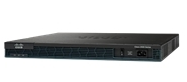
\includegraphics[width=0.5\textwidth]{./images/7.png}
    \caption{Un routeur}
\end{figure}

Les deux routeurs sont redondés pour assurer une pérennité des équipements,
La particularité principale sur la sélection d'un routeur est la fonctionnalité qu'il fasse du Gigabit,
Le SFP est aussi important qui est un module intégré de convertisseur mode fibre, Dans le cas où dans l'ancien bâtiment, il ne dispose pas de cette fonctionnalité pour assurer la fibre optique, il sera préférable de prévoir un achat SFP,

Nous avons sélectionné donc deux routeurs au choix :



    \begin{center}
        \begin{tabular}{|l|p{5cm}|p{5cm}|}
          \hline
            Marque  &   TP-Link : T3700G-28TQ    &   Cisco 2901 \\
          \hline
            Debit  &
Gigabit Ethernet
24 x 10/100/1000 + 4 x SFP Gigabit combiné + 2 x 10 Gigabit SFP
   &   Gigabit Ethernet
10/100/1000
Ethernet, Fast Ethernet, Gigabit Ethernet \\
          \hline

Protocoles supportés
  &   RIP-1, RIP-2, IGMP, VRRP, OSPFv2, PIM-SM, routage IP statique, PIM-DM, ECMP
SNMP 1, RMON 1, RMON 2, RMON 3, RMON 9, SNMP 3, SNMP 2c, HTTP, TFTP, SSH, SSH-2, CLI   &   OSPF, IS-IS, BGP, EIGRP, DVMRP, PIM-SM, IGMPv3, GRE, PIM-SSM, routage statique IPv4, routage statique IPv \\
          \hline
            Performances  &
Capacité de commutation : 128 Gbps
   &
Capacité de commutation : allant 128 Gbps et +
 \\
          \hline
            Tables  &
32 000 entrées
   &
n/c
 \\
          \hline
            Commentaires  &
Conformité aux normes, toutes configurations, controle de flux, DHCP, STP, ACL, VLAN etc,,,
   &
Conformité aux normes, toutes configurations, Cisco IOS Security, controle de flux, DHCP, STP, ACL, VLAN etc,,,
 \\
          \hline
            Dimensions  &
$44 cm * 33 cm * 4,4 cm$
   &
$43,8 cm * 43,9 cm * 4,5 cm$
 \\
          \hline
            Prix
            &
            $1884,11 * 2 = 3768,22  \euro$
            &
            $1909 * 2 = 3818  \euro$
 \\
          \hline
        \end{tabular}
    \end{center}

Une fois les routeurs sélectionnés, le choix des commutateurs avec routage réservés à la distribution, auront pour rôle de répartir chaque trame qui circule dans le réseau, Comme expliqué ci-avant un commutateur avec routage permet d'interconnecter des réseaux homogènes ici dans notre cas : les étages de ce nouveau bâtiment,
Par la suite des commutateur devront être installés au niveau de chaque étage dont un qui est principal qui assure l'ensemble des liens et de la fonctionnalité voix,


\subsubsection{Commutateurs}

Pour continuer, le choix des équipements supplémentaires se portent sur les commutateur qui commuteront des trames, Deux commutateur seront préconisés, En effet redonder un commutateur permet de bien séquencer les trames, éviter les domaines de collisions et assurer la panne matérielle,
Le choix des commutateur se porte principalement sur la capacité à transmettre les trames, Des ports de haut débit permettront d'améliorer le débit de transit reliés au routeur,

\begin{figure}[!ht]
    \center
    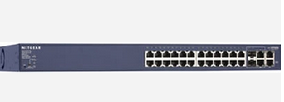
\includegraphics[width=0.5\textwidth]{./images/10.png}
    \caption{Un commutateur}
\end{figure}

Nous prévoyons 2 commutateurs supplémentaires par étage pour assurer la disponibilité,

Nous proposerons 2 commutateurs au choix afin de ne pas se focaliser sur un matériel a proprement dit,
Nous allons structurer le choix des matériels par étage :
A l'étage N-1 : étage critique nous avons  besoin d'un seul commutateur de niveau 2 et 24 ports pour l'ensemble des terminaux,


    \begin{center}
        \begin{tabular}{|l|p{4cm}|p{4cm}|p{4cm}|}
          \hline
            Marque  &  TP-Link TL-SG3424 &   CISCO SF220-24 &  Netgear FS728TPv1 \\
          \hline

Nombre de ports
  &   24 x 10/100 + 2 x combo Gigabit SFP
    &   24 x 10/100 + 2 x combo Gigabit SFP
24 x 10Base-T/100Base-TX - RJ-45
24 x 10Base-T/100Base-TX - RJ-45 - PoE
2 x 10Base-T/100Base-TX/1000Base-T - RJ-45
2 x SFP  & 24 ports Ethernet
4 ports Gigabit
Multicast VLAN Registration \\
          \hline
            Dimensions  &   $440 * 330 * 44 mm $                       &   $440 * 201 * 44 mm$ & $440 * 257 * 44 mm$                 \\
          \hline
            Prix  &
$224,90 \euro   $
    &
$214,90  \euro   $
 &
$269,90  \euro   $
 \\
          \hline
        \end{tabular}
    \end{center}

Pour l'étage N1, il faut 2 commutateur de 24 ports chacun pour raccorder l'ensemble des téléphones IP des postes ainsi que des bornes Wifi,
Revenons au tableau de l'étage N-1 le choix peut se faire suivant les caractéristiques de ces deux matériels choisis,
Chacun d'eux supporte bien évidemment la voix et à des caractéristiques appréciables,
Prenons donc l'hypothèse du choix du commutateur CISCO de 24 ports chacun, pour cela il faut débourser la somme de $214,90 \euro    X 2 = 429,80  \euro$.

Pour les étages N2 à N4 il faut 2 commutateur 24 ports,
Nous gardons l'hypothèse du commutateur CISCO de 214,90  \euro    sachant qu'il en faut deux par étage il en faut donc 6 au total,
Or nous privilégions un surplus en cas de panne majeure et pouvoir les remplacer,
Deux commutateurs supplémentaires semble suffisant,
Un total de $214,90 * 6 + 214,90 * 2 = 2369,20  \euro    $



\subsubsection{Serveur lame }

Un serveur lame est un serveur de petite taille facilitant l'installation de celui-ci dans une armoire de brassage,

\begin{figure}[!ht]
    \center
    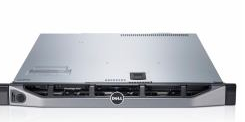
\includegraphics[width=0.5\textwidth]{./images/13.png}
    \caption{Un serveur applicatif}
\end{figure}

L'un des  avantages de ce type de serveur est son coût acquisition,
En effet au fil du temps son retour sur investissement coûte moins cher qu'une exploitation standard de machine serveur,
De plus sa mise en place est bien plus rapide et efficace,

Nous avons sélectionné deux types de serveur, Le choix s'est porté sur leur caractéristiques et sur leur services rendus,

    \begin{center}
        \begin{tabular}{|l|p{5cm}|p{5cm}|}
          \hline
            Marque  &
Power Edge R220 Dell
    &   DELL PowerEdge R320
 \\
          \hline
Processeur
  &
Intel Xeon
    &
Intel Xeon
 \\
          \hline
Mémoire RAM
  &
8 Go
    &
8 Go
 \\
          \hline
            Caractéristiques  &
4000 gigaoctets 7200 RPM en RAID 1, PERC H310, iDRAC7 Express, DVDRW, 2x GLAN, 250W
                & 16 To, technologie de virtualisation, SATA, RAID, alimentation 350 W
6 coeurs
                  \\
        \hline
            Prix  &
$920.05 * 2 = 1840.10 \euro   $
    &
$1544 * 2 = 3088 \euro   $
 \\
          \hline
        \end{tabular}
    \end{center}

Le choix de ces serveurs lame se caractérise par leur extensibilité pour le futur. En effet si le besoin de mémoire se fait ressentir par exemple, alors il sera possible d'agrémenter des ressources dans ces serveurs. De plus ces serveurs ont un prix abordable pour le besoin souhaité. Il est même possible de faire l'acquisition d'un serveur machine mais sa particularité imposante et limitée en ergonomie ne facilitera pas le retour sur investissement à long terme. Il sera donc nécessaire de les changer dans 5-8 ans.


\subsubsection{Serveur NAS}

Un serveur NAS est un équipement à part entière. Il permet de faire du stockage réseau à grande quantité.
Sa particularité est son coût mais aussi sa forte capacité de stockage.

Le NAS permet à l'ensemble de l'équipe hospitalier de sauvegarder périodiquement un ensemble de données modifiées dans la base de données. Cet accès au stockage permet également de consulter les informations d'un patient par exemple.

\begin{figure}[!ht]
    \center
    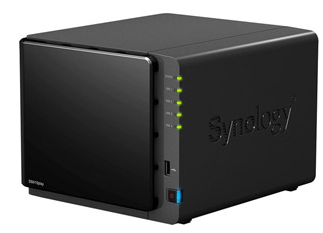
\includegraphics[width=0.5\textwidth]{./images/15.png}
    \caption{Un NAS}
\end{figure}

Nous avons choisi deux NAS aux prix différents. Le choix se fera en fonction du besoin précis de la capacité et au nombre de disques désirés.
Le choix d'un serveur NAS se détermine également par la fonctionnalité du RAID supporté.

RAID 5
le RAID 5 tolère la panne d'un disque dur. Cette particularité du RAID 5 a besoin d'un minimum de 3 disques durs. Contrairement à la copie en miroir, le RAID 5 assure la redondance des informations des disques en stockant les information de parité. Il faut cependant privilégier des disque de même capacité et de même marque si besoin.


    \begin{center}
        \begin{tabular}{|l|p{5cm}|p{5cm}|}
          \hline
            Marque  &
Synology Disk Station DS2415
    &   Synology DiskStation DS415Play
 \\
          \hline
Capacité du NAS
  &
6 disques pour $96To$
    &
4 disque pour $24To$
 \\
          \hline
compatible services réseaux
  &
TCP/ IP, PPTP, PPPoE, iSCS, FTP, NFS, AD webdev, AFP, CalDAV, DHCP, DNS, DDNS, SNMP, Telnet, SSH
    &
TCP/ IP, PPTP, PPPoE, iSCSI, FTP, DHCP, DNS, DDNS, SNMP, Telnet, SSH
 \\
          \hline
            Caractéristiques  &
4000 gigaoctets 7200 RPM en RAID 1, PERC H310, iDRAC7 Express, DVDRW, 2x GLAN, 250W
                & 16 To, technologie de virtualisation, SATA, RAID, alimentation 350 W
6 coeurs
                  \\
        \hline
            Prix avec disques &
$1236 + 139.50 * 12 = 2910 \euro   $
    &
$425 + 226.66 * 4 = 1331.64 \euro   $
 \\
          \hline
        \end{tabular}
    \end{center}


\subsubsection{Onduleur}

Un onduleur est un équipement permettant de sécuriser l'ensemble des équipements inter-connectés. Il s'agit d'un dispositif électronique de forte puissance qui permet de délivrer des tensions et des courants alternatifs à partir d'une source d'énergie électrique continue. De ce fait il préserve l'extinction des équipements.

L'onduleur sélectionné sera branché avec les équipements :
Routeurs
serveurs Lame
NAS

Il nous en faut au moins 5 prises pour les différents équipements.

\begin{figure}[!ht]
    \center
    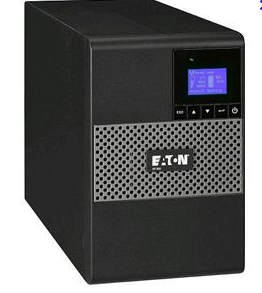
\includegraphics[width=0.4\textwidth]{./images/18.png}
\end{figure}

800 W et comporte 8 prises pour un prix d'environ 300 \euro



\subsubsection{Bornes WiFi}

Concernant les bornes Wi-fi, une borne 2.4Ghz destinée pour les patients est installée sur chaque étage et deux bornes double bande soit 5Ghz destinées pour l'ensemble du personnel pour assurer une continuité d'accès fiable au réseau sans-fil.

\begin{figure}[!ht]
    \center
    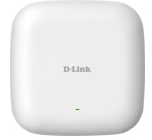
\includegraphics[width=0.5\textwidth]{./images/20.png}
\end{figure}

Un tableau comparatif de bornes Wifi 5 Ghz pour le personnel. Ces bornes sont placées au nombre de deux aux étages :
N0 : Accueil
N1 : Bureaux administratifs
N2 à N4  Chambres des patients
Il faut donc 10 bornes Wi-Fi pour couvrir l'ensemble de ce nouveau bâtiment.



    \begin{center}
        \begin{tabular}{|l|p{5cm}|p{5cm}|}
          \hline
            Marque  & Ubiquiti UniFi AP-Pro UAP-Pro
    &   D-Link DAP-2660
 \\
          \hline
Fréquences supportées
  &
Double radio 2.4 GHz et 5 GHz
    &
Double radio 2.4 GHz et 5 GHz
 \\
          \hline
Protocoles de liaison
  & IEEE 802.11a
IEEE 802.11b
IEEE 802.11g
IEEE 802.11n
    & IEEE 802.11a
IEEE 802.11b
IEEE 802.11g
IEEE 802.11n
 \\
          \hline
            Alimentation  & Compatible PoE & Compatible PoE
                  \\
          \hline
            Nombre de connexions  & $100+$ & $100+$
                  \\
          \hline
            Couverture  & $150m$ & $150m$
                  \\
        \hline
            Prix avec disques &
$221.64 * 10 =2216.4 \euro   $
    &
$298.31 * 10 = 2983.1 \euro   $
 \\
          \hline
        \end{tabular}
    \end{center}

Des bornes Wifi configurées seulement sur la bande 2.4 Ghz servent l'ensemble des visiteurs. Ces bornes sont placées au niveau de chaque étages au nombre d'une borne par étage :
N0 : Accueil;
N2 à N4 : Chambres des patients;
Il en faut quatre bornes Wi-Fi  pour couvrir l'ensemble de ce nouveau bâtiment.



\subsubsection{Baie de brassage}


La question qui se pose : quel est le type de baie de brassage à prendre et à quel nombre ?
Ici chaque équipement du cœur de réseau que nous avons sélectionné pour la solution proposée s'adapte aux baies de brassage de taille standard.
Le choix de sa profondeur est un point essentiel à prendre en compte, il faut cependant savoir aussi que la longueur est importante.

\begin{figure}[!ht]
    \center
    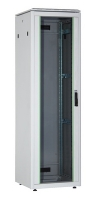
\includegraphics[width=0.3\textwidth]{./images/24.png}
\end{figure}

Il faut donc, cependant prévoir un peu plus large pour l'espace annoncé dans le coeur de réseau. Pour cela, nous prendrons une baie standard de 19 pouces afin que chaque équipement puisse s'intercaler dans chaque compartiments. Nous prenons également une armoire à baie, pour les simples raisons :
Espacement des équipements, facilite l'évacuation de la chaleur
Espace disponible pour de futures installations.
Cette baie sera installée dans le local dédié au coeur de réseau au rez-au-chaussée de l'accueil
Deux baies attirent notre attention pour leur dimension, leur ergonomie, et leur adaptation aux équipements :

    \begin{center}
        \begin{tabular}{|l|p{5cm}|p{5cm}|}
          \hline
            Marque  & LogiLink
    &   DIGITUS
 \\
          \hline
Dimensions
  &
$(L)600 * (P)600 * (H)2.033 mm$
    & $ (L)600 * (P)600 * (H)1.577 mm $

 \\
          \hline
Dimensions tiroirs
  & 19 Pouces standard à tous équipements
    & 19 Pouces standard à tous équipements
 \\
          \hline
            Commentaires   & Porte vitrée, aérations, rehaussement de l'armoire & Porte vitrée, aérations, rehaussement de l'armoire
                  \\
        \hline
            Prix &
$ 578.88 \euro   $
    &
$ 561.13 \euro   $
 \\
          \hline
        \end{tabular}
    \end{center}

Concernant les baies de brassages de chaque niveau, une baies de petite taille suffit car elle accueil seulement deux commutateurs.
Chaque baie sera installée dans un local dédié de chaque étage. Un tableau caractéristique propose deux baies.

\begin{figure}[!ht]
    \center
    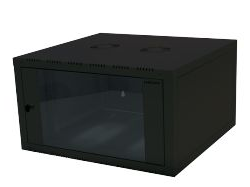
\includegraphics[width=0.5\textwidth]{./images/25.png}
\end{figure}


    \begin{center}
        \begin{tabular}{|l|p{5cm}|p{5cm}|}
          \hline
            Marque  & LogiLink
    &   LogiLink
 \\
          \hline
Dimensions
  &
$(L)600 * (P)560 mm$
    & $ (L)600 * (P)450 mm $

 \\
          \hline
Dimensions tiroirs
  & 19 Pouces
    & 19 Pouces
 \\
          \hline
            Commentaires   & 6U, fixation murale, porte vitrée, aérations & 9U, fixation murale, porte vitrée, aérations
                  \\
        \hline
            Prix &
$ 159.59 * 5 = 797.95  \euro   $
    &
$ 155.03 * 5 = 775.15 \euro   $
 \\
          \hline
        \end{tabular}
    \end{center}





\subsection{Liaison des équipements}

Le choix des câbles n'est pas si facile. En effet plusieurs caractéristiques sont à prendre en compte.

Pour commencer il faut savoir quel type de conducteur est utile.
Le monobrin est constitué de deux fils dont en paire torsadée et une en cuivre massif. Les câbles monobrins peuvent atteindre une portée de 100 mètres et sont destinés à être installés dans des murs ou sous plafond.
Le multibrin est constitué de deux fils également mais d'une paire torsadée mais aussi d'une tresse de micro-fils de cuivre. On les remarque grâce à leur souplesse. Ce type de câble n'est pas similaire au monobrin. En effet le signal est plus atténué. Pour des longueur de moins de 30 mètres il faut les éviter pour éviter ces atténuations.

Le multibrin semble répondre a un environnement professionnel et en gain majeur de transfert.

Il est cependant important de souligner que dans un établissement médical, le type de blindage est à prendre en compte pour en assurer la sécurité. En effet la norme LSZH (Low Smoke Zero Halogene) est obligatoire dans les installations professionnelles dont médicales principalement. Il faut cependant prendre des câbles sans halogène.

Le type de blindage SFTP Shielded Foiled Twisted Pair de Cat6  plus dispose des paires blindées par un écran en aluminium, ainsi la gaine extérieure est aussi blindée par une tresse en cuivre étamé.

Le choix du cable sera donc du cat6a car sa Fréquence inférieur à 500 Mhz et supporte le 10Gbits Ethernet. Ce type de câble permettra d'assurer une certaine évolution si besoin le réseau serait amené à changer.
La catégorie 6 uniquement peut être choisie pour les périphériques finaux  et les étages.

Une longueur raisonnable de 300 mètres de CAT6a devrait couvrir l'ensemble du bâtiment.
Prix : environ $ 268,50 \euro $



\subsection{Climatiseur}

\begin{figure}[!ht]
    \center
    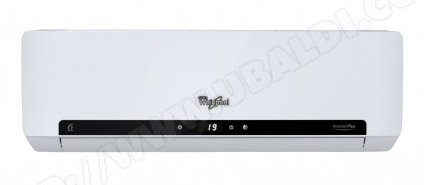
\includegraphics[width=0.4\textwidth]{./images/28.png}
\end{figure}

Garder la pièce du coeur de réseau au frais est important car chaque équipement dégage de la chaleur lors de son fonctionnement. En cas de non respect de la temperature fraiche, des dysfonctionnements d'équipements pourraient survenir. L'ajout d'un climatiseur facilite les équipement à bien fonctionner et à assurer leur activité à long terme.

La température est variable, été comme hiver, ce climatiseur s'adapte à tout type d'environnement.
Cet équipement est important pour assurer une certaine sécurité dans le réseau. Il est évident de dire qu'un réseau bien constitué, peut perdre de ces performances si un climatiseur est inexistant.
Prix : environ $ 601 \euro $



\subsection{Terminaux}

\subsubsection{Ordinateurs}



    \begin{center}
        \begin{tabular}{|l|p{2cm}|p{2cm}|p{2cm}|p{2cm}|}
          \hline
            Caractéristiques  & Ordinateur & Écran & clavier / souris & lecteur de carte vitale \\
          \hline
            Marque  & DELL Ordinateur de bureau Vostro & Philips 18.5" LED - 193V5LSB2 & Dell & Ingenico Xiring \\
        \hline
            Prix &
$ 349 * 21 = 8765.4 \euro   $
    &
$ 85.95 * 21 = 4211.95 \euro   $
    &
$ (14.79 + 18.48) * 21 = 1630.23 \euro   $
    &
$ 229 * 12 = 2748 \euro   $
 \\
          \hline
        \end{tabular}
    \end{center}



\subsubsection{Téléphones}

\begin{figure}[!ht]
    \center
    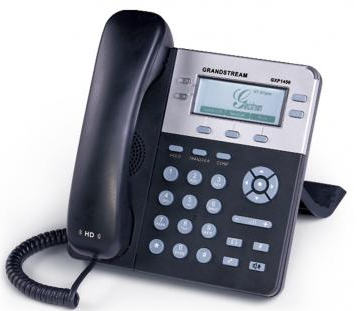
\includegraphics[width=0.4\textwidth]{./images/29.png}
\end{figure}

Les téléphones VOIP fixe destiné aux personnels sont du modèle GXP1450 HD Grandstream.
Ce téléphone à les fonctionnalités suivante: DECT 4 appels simultanés, groupement d'appels, appel entrant, attente, codec vocaux, service sécurisé HTTPS/TFTP/SRTP et dispose d'un écran LCD . Il est raccordable via une interface RJ45 et supporte la technologie PoE. Ils faut 32 téléphones afin de répondre au besoin de la clinique. Le coût unitaire est de 54.43 \euro.

Les téléphones destinés au patients sont eux moins sophistiquer, il n'y a pas d'écrans LCD et ne supporte pas toutes les options cité ci-dessus. Il est aussi raccordé en RJ45 et supporte le PoE.

\begin{figure}[!ht]
    \center
    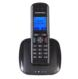
\includegraphics[width=0.2\textwidth]{./images/31.png}
\end{figure}

Pour finir les téléphones sans fil pour le personnel est aussi de la marque GrandStream, et de modèle DP715
Il a les même caractéristique que le téléphones filaire pour le personnel. sont socle doit être à 50 mètres du téléphone.
Son autonomie est de 10h. Le prix unitaire est de 139.95 \euro.


\begin{figure}[!ht]
    \center
    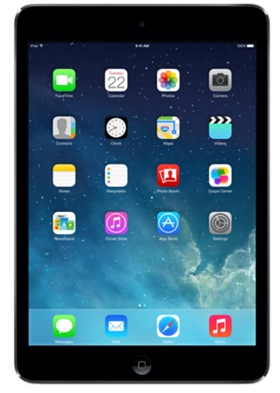
\includegraphics[width=0.3\textwidth]{./images/32.png}
\end{figure}

Les tablettes misent à disposition du personnel sont de la marque Apple et de modèle Ipad Mini. Son autonomie est de 10h et son prix de 300 \euro.




\subsection{Devis}

\begin{itemize}
\item 32 Téléphone VOIP Fixe Personnel (54.43 \euro) : 1741.76\euro ;
\item 60 Téléphone VOIP Fixe Patients (46.90 \euro) : 4221\euro ;
\item   9 packs de 3 Téléphones VOIP sans fil (139.95 \euro )   : 1259.55\euro;
\item  15 Ipad mini 2 Tablette (299 \euro)   : 4489\euro;
\item  28 Ordinateur Médecin (547\euro )   : 18317.936\euro;
\item   21 ordinateur Administratif (349\euro)   : 8765.484\euro;
\item   49 Ecran ordinateur (85.95\euro)   : 4211.55\euro ;
\item   49 Clavier + Souris (33.27\euro)   : 1630.23\euro;
\item  12 Outil carte vitale (229\euro)   : 2748\euro;
\item   300m de Fibre Optique : 369,42 \euro ;
\item  6 + 6 Connecteurs Fibre Optique SFP + SC (22.24 \euro + 6.02 \euro)   : 339.12\euro;
\item     2  Routeur TP-Link : T3700G-28TQ      (1884.11\euro)            :    3768.22\euro    ;
\item       2  Serveur lame Power Edge R220 Dell    (920.05 \euro)            :   1840.10\euro     ;
\item      NAS 48 To avec 12 disques   (1236 \euro + 1674 \euro)            :    2910\euro     ;
\item        Onduleur               :       309.60 \euro  ;
\item          15 Switch Cisco 24p        (214,90 \euro)   :    3223.5\euro     ;
\item              Etage N0 Switch Netgear FS728TPv1 24p       :    269.90\euro     ;
\item        10   kit de mise en rack  (10\euro)            :     100\euro    ;
\item         20  D-Link DAP-2660 (298,31 \euro)            :     5966.2 \euro    ;
\item          Baie de brassage coeur de réseau Logilink          :      578.88 \euro   ;
\item          5 Baie de brassage Etage  (159.59 \euro)            :     797.95\euro    ;
\item            Cable CAT6a 300m          :      216,00\euro   ;
\item            Climatiseur coeur de réseau          :     601\euro    .
\end{itemize}

Le prix annoncé de 67991.45\euro  rassemble donc tous les critères de configurations explicité dans ce document.



%

    \cleardoublepage
    %
    \section*{Conclusion}
\addcontentsline{toc}{section}{Conclusion}

Pour conclure, avec \LaTeX{} on obtient un rendu impeccable mais il faut s'investir pour le prendre en main.

    \cleardoublepage
    %
    %~ \phantomsection\addcontentsline{toc}{section}{Références}
%
\begin{thebibliography}{ABC}
    %
    \bibitem[REF]{reference} auteur. \emph{titre}. édition, année.
    %
    \bibitem[LPP]{lpp} Rolland. \emph{LaTeX par la pratique}. O'Reilly, 1999.
%
\end{thebibliography}

    %
\end{document}
